\documentclass{article}
\usepackage[utf8]{inputenc}
\setlength{\parindent}{0pt}
\addtolength{\hoffset}{-3cm}
\addtolength{\textwidth}{6cm}
\usepackage[francais]{babel}
\usepackage{fontspec}
\usepackage{amsmath}
\usepackage{amsfonts}
\usepackage{xcolor,graphicx}
\usepackage{minted}
\usemintedstyle{colorful}
\usepackage{float}

\title{Kernel TP3 - Rapport système de fichiers - TexFS}
\author{Maxime Lovino \and Loic Willy}

\begin{document}
\maketitle
\newpage
\section{Introduction}
Pour réaliser le système de fichiers utilisé par notre Kernel, nous nous sommes inspirés du système de fichiers Ext2 sur lequel nous avons travaillé pendant un semestre en deuxième année. Nous avons adapté Ext2 par rapport aux besoins qui étaient spécifiés pour ce projet. C'est-à-dire que nous avons principalement simplifié Ext2 en supprimant les doubles et triples indirections, qui ne sont pas nécessaires compte tenu de la taille des fichier que nous devons stocker. Nous n'avons également pas tenu compte de la notion de groupes.\\

De ce fait, lors de la création d'une image TexFS, il est nécessaire de spécifier la taille de bloc, le nombre de bloc à allouer et le nombre de fichiers maximum pour l'image. La taille de bloc et le nombre de blocs devaient être spécifiés de toute façon, mais compte tenu de la structure utilisée, il est nécessaire d'entrer également le nombre de fichiers maximum que contiendra l'image. (Si nous avions des groupes, nous aurions pu allouer un nouveau groupe en cas de besoins de nouveaux fichiers)
\section{Structure du système de fichiers}
TexFS a une structure sur le disque similaire à Ext2. Nous n'avons par contre pas besoin de réserver le premier block pour le MBR car nous ne démarrons pas sur notre image. Du coup nous commençons au block 0 par le superblock, suivi du block bitmap, puis de l'inode bitmap et de la table des inodes. Après toutes ces blocs de métadonnées, nous avons les blocs de données.
\begin{figure}[H]
    \centering
    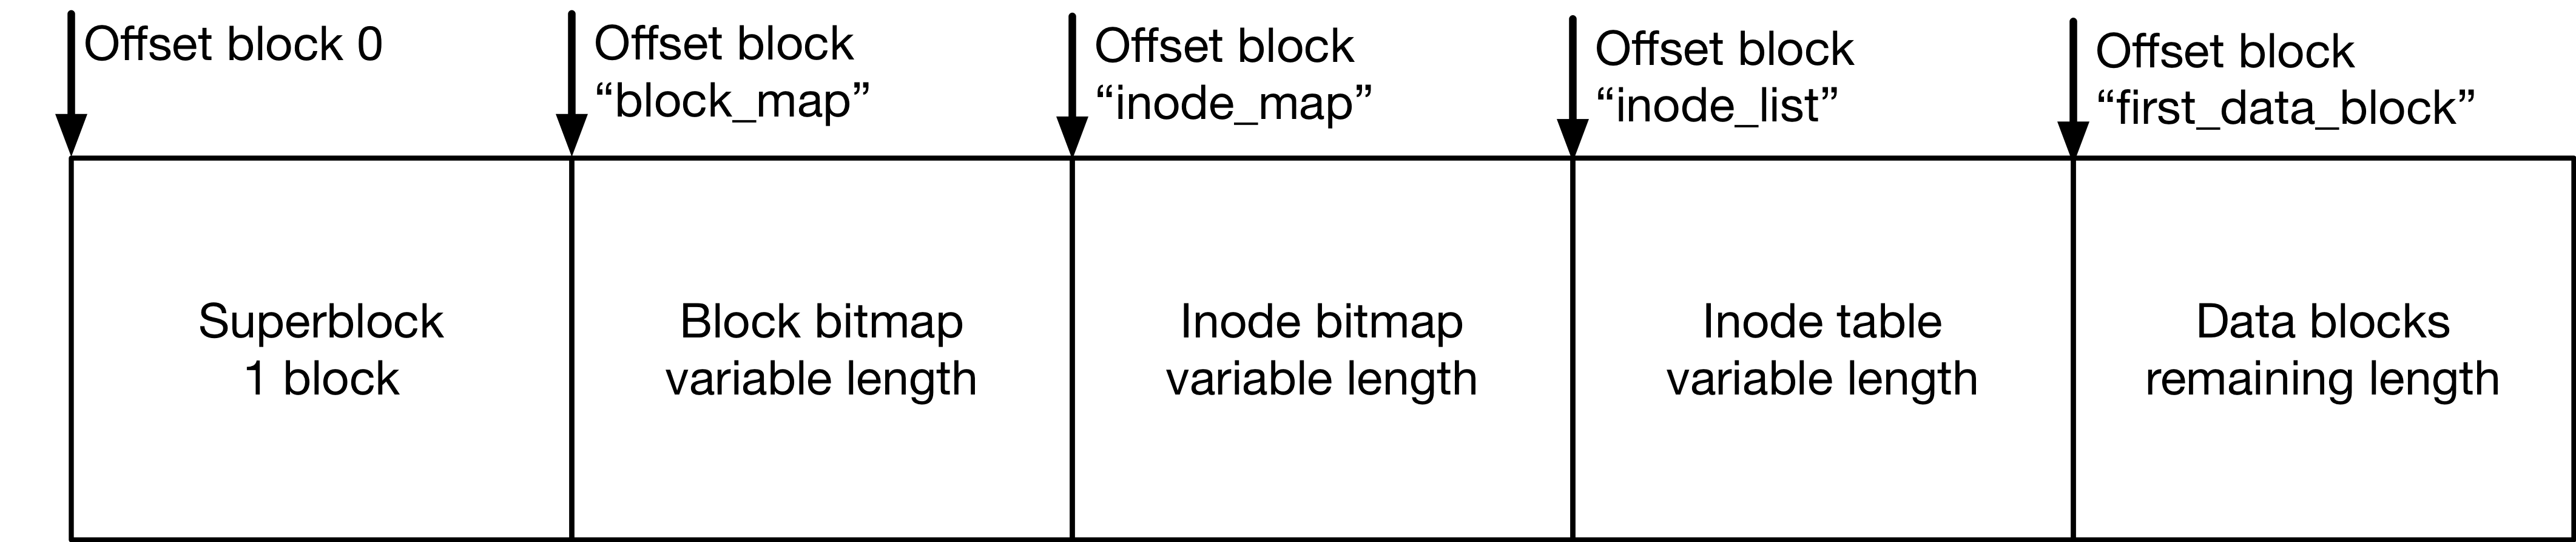
\includegraphics[width=\textwidth]{FS_disk_structure.png}
\end{figure}
\subsection{Blocs de métadonnées}
Cette section va rentrer plus en détail sur les blocs de métadonnées, étant donné que les blocs de données sont juste composées de données brutes ou d'index de blocs indirects (expliqué plus loin).
\subsubsection{Superblock}
\begin{minted}[breaklines,breaksymbol=, linenos, frame=single, stepnumber=5,tabsize=2]{C}
#define MAX_LABEL_LENGTH 30
typedef struct tex_fs_superblock_st {
    uint16_t magic;
    uint8_t version;
    char label[MAX_LABEL_LENGTH];
    uint16_t block_size;
    uint32_t block_map;
    uint32_t block_count;
    uint32_t inode_bitmap;
    uint32_t inode_list;
    uint32_t inode_count;
    uint32_t first_data_block;
} __attribute__((packed)) tex_fs_superblock_t;	
\end{minted}
Le superblock comprend le \verb+magic+ de TexFS, c'est-à-dire \verb+0xD0D0+ ainsi que la version du filesystem (version 1) et le label choisi à la création de l'image. Ensuite le champ \verb+block_size+ nous permet d'avoir la taille des blocs, à noter qu'il s'agit d'un entier signé sur 16 bits, du coup nous avons une taille de bloc maximale de $2^{16}-1=65535$ bytes, ce qui est suffisant dans notre cas. \\

Ensuite, \verb+block_map+, \verb+inode_bitmap+, \verb+inode_list+ et \verb+first_data_block+ représentent les numéros de blocks à laquelle commencent les sections correspondantes. \verb+block_count+ et \verb+inode_count+ représentent respectivement le nombre de blocks de l'image et le nombre d'inodes.
\subsubsection{Block bitmap et inode bitmap}

\subsubsection{Inode Table}
\begin{minted}[breaklines,breaksymbol=, linenos, frame=single, stepnumber=5,tabsize=2]{C}
#define DIRECT_BLOCKS 8
#define INDIRECT_BLOCKS 4
#define MAX_FILENAME_LENGTH 64
typedef struct tex_fs_inode_st {
    char name[MAX_FILENAME_LENGTH];
    uint32_t size;
    uint32_t direct_blocks[DIRECT_BLOCKS];
    uint32_t indirect_blocks[INDIRECT_BLOCKS];
} __attribute__((packed)) tex_fs_inode_t;
\end{minted}
L'inode contient toutes les métadonnées d'un fichier ainsi que les indices des blocs directs et indirects qui contiennent les données de ce fichier. En terme de métadonnées, on stocke la taille et le nom (maximum 64 char). \\

On a 8 blocs directs et 4 blocs indirects. En se basant sur le fait que chaque indice de bloc est stocké sur 4 bytes, on peut calculer la taille maximum d'un fichier en fonction de la taille d'un bloc $n$, on obtient $8 * n + (4 * \frac{n}{4} * n)$. Pour une taille de bloc minimale de 512 bytes, on peut stocker un fichier de taille $8 * 512 + (4 * \frac{512}{4} * 512)=266240$ bytes, ce qui est suffisant par rapport à la taille demandée de 256 kbytes.\\

Les données des blocs directs sont stockés de cette façon: \\
\begin{figure}[H]
	\centering
	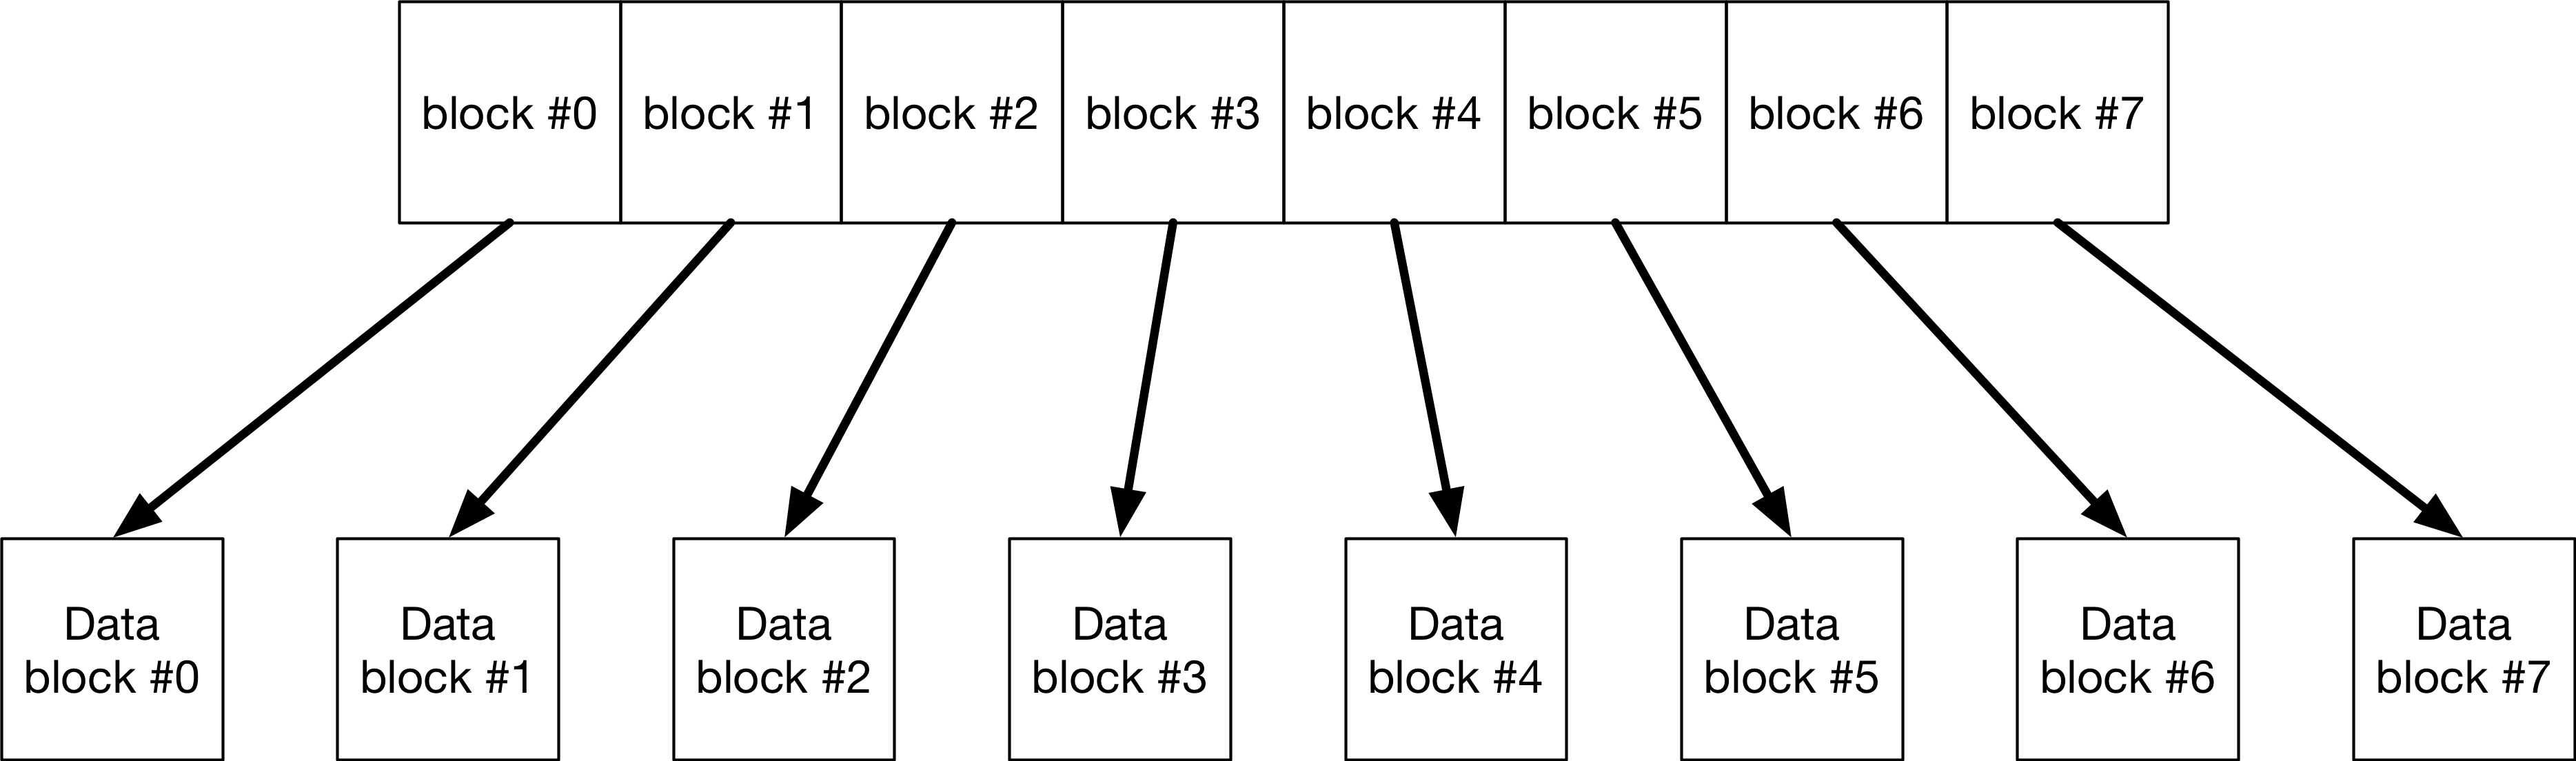
\includegraphics[width=\textwidth]{FS_direct.png}
\end{figure}

Les données des blocs indirects sont elles stockées de cette façon: \\
\begin{figure}[H]
	\centering
	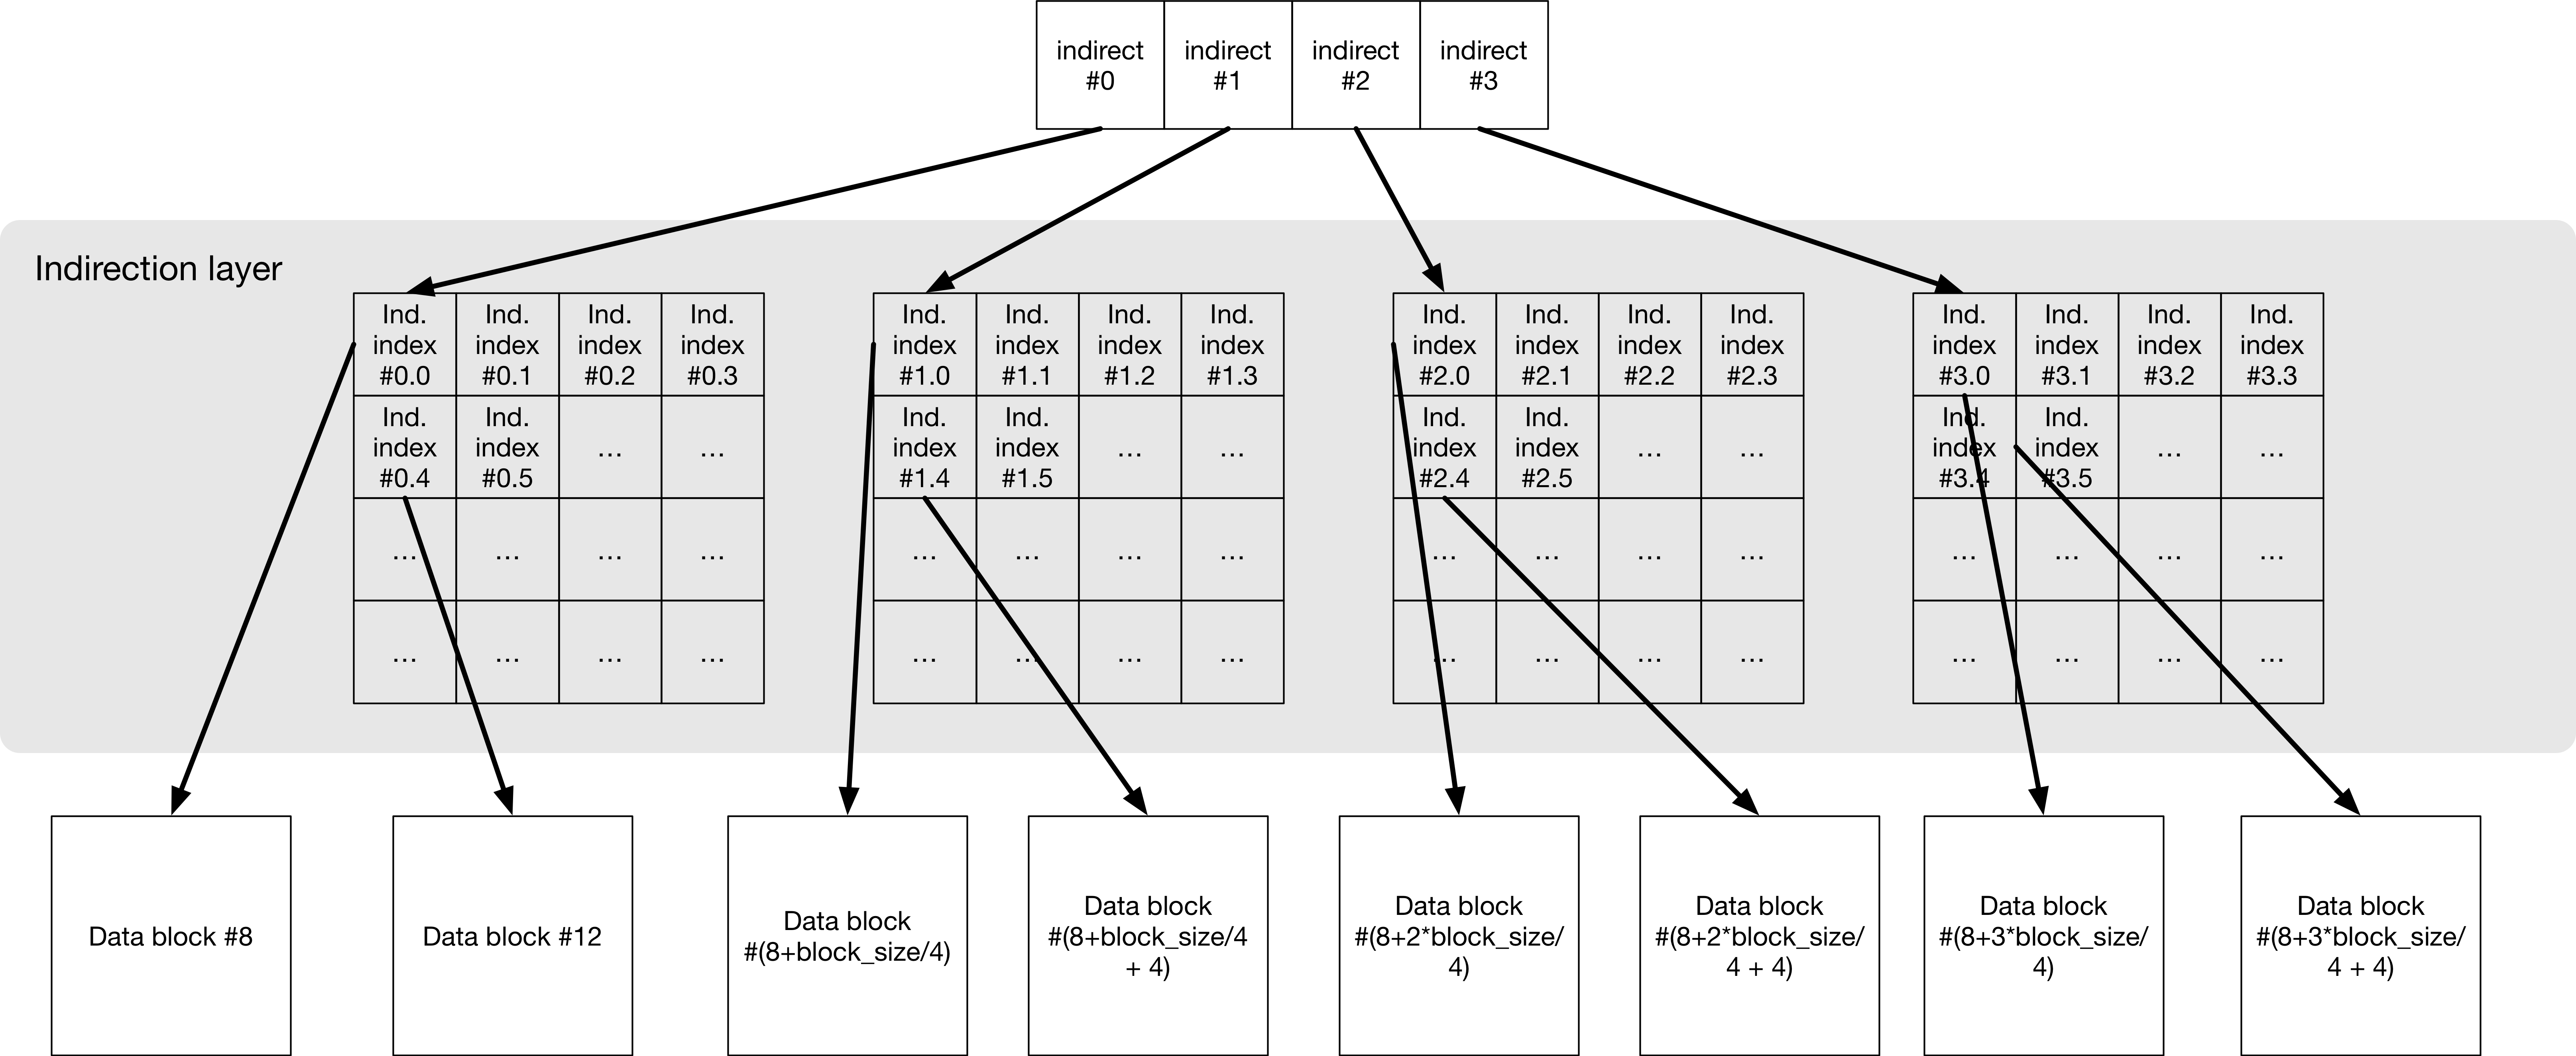
\includegraphics[width=\textwidth]{FS_indirect.png}
\end{figure}
\section{Exemples}
\section{Implémentation}
\section{Avantages du système choisi}
\begin{itemize}
	\item Structure inspirée de Ext2, donc déjà connue
	\item Séparation des métadonnées et données
	\item Facile de stocker toutes les métadonnées en RAM
	\item La bitmap d'inodes et de blocks permet de trouver facilement des inodes et blocks libres
	\item Itération sur les fichiers simple (il suffit de prendre la prochaine inode utilisée)
	\item Les fichiers peuvent facilement grandir
	\item Accès aléatoire dans un fichier rapide (accès direct si block direct, lecture d'un bloc indirect puis accès direct si indirection)
	\item Pas de fragmentation externe
\end{itemize}
\section{Inconvénients du système choisi}
\begin{itemize}
	\item Retrouver tous les blocks d'un fichier avec indirections est compliqué
	\item Cela influe sur la lecture et la suppression d'un fichier
	\item Pour itérer sur les fichiers, il faut parcourir toutes les inodes
	\item Overhead de stockage pour les blocks métadonnées
	\item Fragmentation interne dans certains blocks (superblock par exemple)
	\item L'accès séquentiel n'est pas plus rapide que l'accès aléatoire, car les blocks de données ne sont pas forcément contigus
\end{itemize}
\end{document}
